\documentclass[main.tex]{subfiles}
 
\begin{document}

\part{Depth of the tremor source}

\chapter{Introduction}

General question - Description of tremor and slow slip

Specific question - Depth of the low-frequency earthquake on the plate boundary. More difficult for the tremor because no phase onset

Previous study La Rocca et al. 2009

Part of the specific question - If the source is on the plate boundary, you should have a constant time lag between P-wave and S-wave arrivals, and a peak in the cross correlation between the vertical component and the horizontal component.

Explain here why it is going to work (No problem with tremor streaks)

\chapter{Data}

The data were collected during the Array of Arrays experiment. Eight small-aperture arrays were installed in the northeastern part of the Olympic Peninsula, Washington. The aperture of the arrays was about 1 km, and station spacing was a few hundred meters. The arrays were around 5 to 10 km apart from each other (Figure 1). Most of the arrays were installed for more than a year, between June 2009 to September 2010, and were able to record the main August 2010 ETS event. Ghosh \textit{et al.} (2012 ~\cite{GHO_2012}) used a multibeam-backprojection (MBBP) technique to detect and locate tremor. They bandpass filtered the seismic data between 5 and 9 Hz. They divided the data into one-minute-long sliding independent (no overlap) time windows. They performed beam forming in the frequency domain at each array to determine the slowness vectors, and backprojected the slownesses in the 3-D space to locate the source of the tremor for each time window. We thus have a catalog of 28902 one-minute-long time window during which tremor was detected. For each time window, we have the beginning time, the end time, and the location (latitude and longitude) of the source of the tremor.

\begin{center}
\includegraphics[width=19cm, trim={0cm 2.5cm 0cm 9.5cm},clip]{Figures/timelags/arrays_location.eps}
\captionsetup{type=figure}
\captionof{figure}{Map showing the location of the eight arrays (red dots) used in this study. Blue dots are the locations of the source of the tremor recorded by the arrays. Inset shows the study area with the box marking the area covered in the main map. Contour lines represent a model of the depth of the plate interface [McCrory \textit{et al.}, 2006 ~\cite{MCC_2006}].}
\end{center}

\chapter{Method}

Grid cells

Cross correlation HV
Stack cross correlation over arrays

Stack cross correlation over time windows

peak about 5-6 s

Divide time windows into two clusters based on

New stack with only the good one

One image here to show the stacking

Time lag betwee direct P and direct S wave

Velocity model -> tremor depth

\chapter{Results}

use all data

Quality of depth

Some sort of least square regression

One image here to show the depth

\chapter{Discussion / Conclusion}

Where are the other tremor? Not wee located? Not on the plate boundary?

How analysis addresses the part of the specific question

How analysis addresses the specific question

How analysis addresses the general question

\end{document}
